\documentclass[9pt]{beamer}
\usetheme{Warsaw}
\usepackage[utf8]{inputenc}
\usepackage[english]{babel}
\usepackage{amsmath}
\usepackage{amsfonts}
\usepackage{amssymb}
\usepackage{graphicx}
\usepackage{fontspec}
\newfontfamily\cjkfont{Noto Sans CJK SC} % Or any appropriate font you have
\author{leviathan/talamon}
\title{Libre Silicon Alliance}
\setbeamercovered{transparent} 
\setbeamertemplate{navigation symbols}{} 
\logo{lsa.png} 
%\institute{} 
%\date{} 
\subject{A free semiconductor manufacturing standard}
\begin{document}

\begin{frame}
	\titlepage
	\begin{center}
		
\includegraphics[width=50pt,height=50pt]{lsa.png}
	\end{center}
\end{frame}

%\begin{frame}
%\tableofcontents
%\end{frame}

\section[What]{}
\begin{frame}{What we do}
	\begin{itemize}
		\item Breaking the monopoly of big semiconductor manufacturers
		\item Eliminating the vendor lock-in to big semiconductor manufacturers
		\item Making semiconductor development super quick and inexpensive
	\end{itemize}
\end{frame}

\section[Who]{}
\begin{frame}{Community projects}
	\begin{center}
		
\includegraphics[width=100pt]{Icarus.png}
		
\includegraphics[width=100pt]{Yosys.png}
		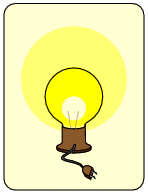
\includegraphics[height=50pt]{Opencircuit.png}
	\end{center}
\end{frame}

\begin{frame}{Companies and institutions}
	\begin{center}
		
\includegraphics[width=100pt]{HKUST_Logo.png}
		
\includegraphics[width=100pt]{NFF.jpg}
		
\includegraphics[width=100pt]{efabless_logo.png} \\
		
\includegraphics[width=100pt]{Lanceville.png}
	\end{center}
\end{frame}

\section[How]{}
\begin{frame}{How we do it}
	\begin{itemize}
		\item Introducing an open source chip manufacturing process standard specification
		\item Introducing a fully integrated free EDA for ASIC design\footnotemark
	\end{itemize}

	\footnotetext[1]{https://github.com/leviathanch/qtflow}
\end{frame}

\section[Why]{}
\begin{frame}{Why are we doing this?}
	\begin{itemize}
		\item MPWs cost around 20'000 USD nowadays
		\item MPWs take around 2-9 months nowadays
		\item All manufacturers want NDAs (some NDAs even have NDAs!)
		\item You design for a vendor process contains process specific design quirks (also under NDA!)
		\item No manufacturer provides the GDS2 files in order to manufacture the designs in your basement (there is \textbf{no} free silicon yet)
		\item You can't even publish your own designs!
	\end{itemize}
\end{frame}

\section[Conclusion]{}

\begin{frame}{Help needed}
	\begin{itemize}
		\item Work on developing QtFlow\footnotemark
		\item Work on the LibreSilicon process\footnotemark
		\item Work on the standard logic cells
		\item Work on developing FreeFLASH
		\item Work on developing FreeDRAM
		\item Financial contributions/Investments
	\end{itemize}

	\footnotetext[2]{https://github.com/leviathanch/qtflow}
	\footnotetext[3]{https://github.com/leviathanch/libresiliconprocess}
\end{frame}

\begin{frame}{Thank you!}
	\begin{center}
		\textbf{Thank you very much!} \\
		\textbf{Vielen herzlichen Dank!} \\
		\textbf{\cjkfont 非常感谢你!} \\
		
\includegraphics[width=100pt]{cat.png}
	\end{center}
\end{frame}

\end{document}